\originalchapter{可解释性与因果干预}\label{ch:interp}
\originalsection{解释要能预测什么}
可解释性首先是一个具体问题: 哪个输入或内部变量改变会怎样影响模型行为? 一张漂亮热力图、一个可读标签或一段模型自述都可能帮助形成假说, 但不能单独成为机制真值. 一个解释若能准确预测尚未观察的反事实行为, 比只复述已知输出提供更多证据.

\begin{definition}
本书区分相关性、可解码性与因果效应. 相关性指两变量统计相关; 可解码性指一个读取函数可以从表征预测某标签; 因果效应指在明确保持其他条件的干预下, 改变变量引起行为差异. 三者没有无条件等价关系.
\end{definition}
例如某隐单元包含输入颜色, 一个线性 probe 能读出颜色, 但最终分类头可能完全不使用它. 也可能多个单元冗余表示同一信息, 消融一个不影响预测. 因而“能读出”不必然“被用于决定”,“消融无效”也不必然“从未参与”.

\originalsection{梯度与积分归因}
对可微标量输出 $f(x)$, 小输入扰动 $\delta$ 给出 $f(x+\delta)-f(x)\approx\nabla f(x)^\top\delta$. 梯度刻画局部敏感性. 对线性 logit $f(x)=w^\top x+b$, 梯度恰为 $w$. 若归因解释的是概率 $\sigma(f(x))$, 则梯度为 $\sigma(f)(1-\sigma(f))w$. 在概率饱和时梯度小, 不意味着输入不重要.

选一个基线 $x_0$, 定义积分梯度
\[
\operatorname{IG}_j(x;x_0)=(x_j-x_{0j})\int_0^1
 \frac{\partial f(x_0+t(x-x_0))}{\partial x_j}\,dt.
\]
若 $f$ 在这条线段上连续可微, 沿线的链式法则和微积分基本定理给出
\begin{align*}
\sum_j\operatorname{IG}_j(x;x_0)
 &=\int_0^1\nabla f(x_0+t(x-x_0))^\top(x-x_0)\,dt\\
 &=f(x)-f(x_0).
\end{align*}
这叫完整性, 是归因和输出差值的数学关系. 它不证明基线选择正确, 也不证明线段经过的输入在真实数据分布中合理. 对离散文本, 在 embedding 间插值更需要解释对象与分布外问题.

\originalsection{消融、替换与匹配对照}
消融将某输入或隐单元置零, 但零可能是训练时从未出现的状态. 用训练均值或另一自然样本的匹配激活替换, 可以减少部分分布外扰动, 却仍不保证只改变一项语义因素. 必须说明被固定和被改变的变量, 再用同范数随机扰动或随机单元组作为对照.

本项目的快捷特征实验有已知数据生成机制. 两特征 Logistic 模型的 logit 梯度就是已训练权重. 若快捷特征权重大, 输入替换也显著改变预测, 可说明模型依赖此特征. 同分布正确率高却在反相关偏移中失效, 则提示依赖与部署目标不匹配. 这仍是输入层面证据, 没有检查大语言模型内部神经元.\par

\begin{figure}[ht]
\centering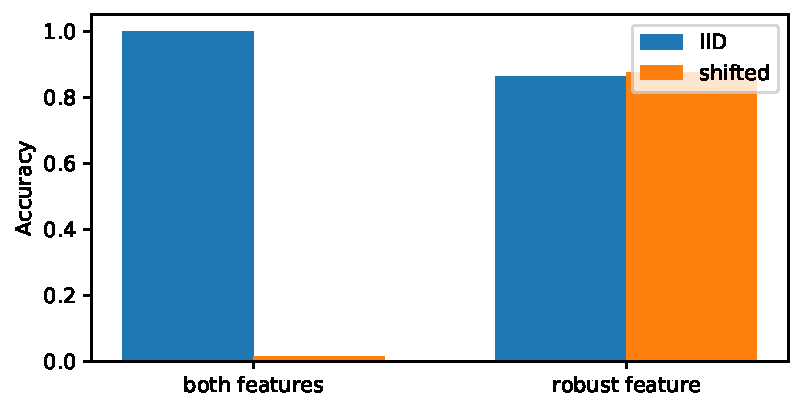
\includegraphics[width=.66\textwidth]{generated/spurious.pdf}
\caption{原创合成特征实验中的同分布与反相关偏移测试. 两种模型各用相同的训练样本与固定更新次数.}\label{fig:shift}
\end{figure}

后续可以训练一个含隐层的模型, 仅用开发集挑出与快捷特征高相关的单元, 然后在独立测试中比较候选单元消融、随机单元消融与输入翻转. 这一步在首版仍是研究计划, 没有把它写成已执行结果.

\originalsection{稀疏特征与前沿证据}
稀疏自编码器试图把激活 $h$ 表示为少量字典方向的组合: $z=\operatorname{ReLU}(W_eh+b_e)$, $\hat h=W_dz+b_d$, 训练目标包含重建误差与稀疏惩罚, 如 $\norm{h-\hat h}^2+\lambda\|z\|_1$. 这里用 $\|z\|_1$ 表示 $\sum_j|z_j|$. 方向更可读不自动表示解释完备; 重建误差、字典冗余、特征分裂与未捕获计算都会影响结论.

2025 年 On the Biology of a Large Language Model 通过替代模型、归因图与干预, 给出部分精选语言模型行为的局部电路证据\cite{biology}. 原文也强调可解释范围有限, 只有部分尝试得到令人满意的洞见, 替代模型不完全等于原模型. 因而应读成“某些案例得到有干预支持的解释”, 不能读成“已全面理解 AI”.

2026 年 CHIVE 把解释质量与反事实行为预测联系起来. 作者在其设置中没有观察到所研究激活读取工具相对只看对话基线的增量提升\cite{chive}. 这提供重要负结果, 不等于所有可解释性研究无用. 2026 年全局工作空间研究给出可言语化表征与若干功能机制的干预证据\cite{workspace}; 它也不证明主观体验、感情或意识. 函数机制、认知理论类比与主观体验证据是不同层次.

\originalsection{练习与解答}
\begin{exercise}
模型为 $f(x_1,x_2)=x_1$, 数据却总满足 $x_2=x_1$. 能否从 $x_2$ 完美预测输出? 这是否说明模型使用 $x_2$?
\end{exercise}
\begin{solution}
在该观测分布上, $x_2$ 完美预测输出. 但保持 $x_1$ 固定、只改变 $x_2$ 时 $f$ 不变, 所以模型的函数并不使用 $x_2$. 相关性不能替代干预. 还要承认该干预离开了原来的数据支撑集合, 真实场景是否允许它需要另行解释.
\end{solution}
\begin{exercise}
对 $f(x)=w^\top x+b$, 求基线为 $x_0$ 的积分梯度, 并检查完整性.
\end{exercise}
\begin{solution}
每个偏导恒为 $w_j$, 所以 $\operatorname{IG}_j=w_j(x_j-x_{0j})$. 求和得到 $w^\top(x-x_0)=f(x)-f(x_0)$. 截距不被分配给输入差值, 与完整性相容.
\end{solution}
\label{ch:end:12}
